\documentclass[12pt]{article}
\usepackage[none]{hyphenat}
\usepackage{amsmath}
\usepackage{float}
\usepackage{graphicx}
\usepackage{atbegshi}
\AtBeginDocument{\AtBeginShipoutNext{\AtBeginShipoutDiscard}}
\newcommand{\solution}{\noindent \textbf{Solution: }}
\providecommand{\brak}[1]{\ensuremath{\left(#1\right)}}
\newcommand{\myvec}[1]{\ensuremath{\begin{pmatrix}#1\end{pmatrix}}}
\let\vec\mathbf
\begin{document}
\graphicspath{{./Documents}{./figs}}
\begin{center}
	\title{\textbf{Straight Lines}}
	\date{\vspace{-5ex}}
	\maketitle
\end{center}
\setcounter{page}{1}
\section*{11$ ^{th} $ Maths - Chapter 10}
The following problem is question 09 from exercise 10.4:
\begin{enumerate}
	\item Find the value of $\vec{p}$ so that the three lines $ 3x + y - 2 = 0, px + 2y - 3 = 0 $ and $ 2x - y - 3 = 0 $ may intersect at one point.
\end{enumerate}
\solution \\
Given equations can be written in the form of $ \vec{n}^{\top}\vec{x} = c$ \\
Therefore, \\ 
\begin{align}
	\myvec{3&1}\vec{x}=2
	\label{eq:1}
\end{align}
\begin{align}
	\myvec{2&-1}\vec{x}=3
	\label{eq:2}
\end{align}
\begin{align}
	\myvec{p&2}\vec{x}=3
	\label{eq:3}
\end{align}\\
Matrix form of above equations \eqref{eq:1}, \eqref{eq:2} and \eqref{eq:3} is
\begin{align}
	\begin{pmatrix}
		3 & 1 \\ \\ 2 & -1 \\ \\ p & 2
	\end{pmatrix}
	\begin{pmatrix}
		x \\ \\ y
	\end{pmatrix}
	=
	\begin{pmatrix}
		2 \\ \\ 3 \\ \\ 3
	\end{pmatrix}
\end{align}
augmented matrix is
\begin{align}
	\begin{pmatrix}
		3 & 1 & 2 \\ \\
		2 & -1 & 3 \\ \\
		p & 2 & 3
	\end{pmatrix}
\end{align}
$ R_1 \rightarrow R_1 + R_2 $
\begin{align}
	\begin{pmatrix}
		5 & 0 & 5 \\ \\
		2 & -1 & 3 \\ \\
		p & 2 & 3
	\end{pmatrix}
\end{align}
$ R_1 \rightarrow \frac{R_1}{5} $
\begin{align}
	\begin{pmatrix}
		1 & 0 & 1 \\ \\
		2 & -1 & 3 \\ \\
		p & 2 & 3
	\end{pmatrix}
\end{align}
$ R_2 \rightarrow R_2 - 2R_1 $
\begin{align}
	\begin{pmatrix}
		1 & 0 & 1 \\ \\
		0 & -1 & 1 \\ \\
		p & 2 & 3
	\end{pmatrix}
\end{align}
$ R_3 \rightarrow R_3 - pR_1 $
\begin{align}
	\begin{pmatrix}
		1 & 0 & 1 \\ \\
		0 & 1 & -1 \\ \\
		0 & 2 & 3-p
	\end{pmatrix}
\end{align}
$ R_3 \rightarrow R_3 - 2R_2 $
\begin{align}
	\begin{pmatrix}
		1 & 0 & 1 \\ \\
		0 & 1 & -1 \\ \\
		0 & 0 & 5-p
	\end{pmatrix}
\end{align}
Therefore, to satisfy Echelon form the bottom row must be zero. Then,
\begin{align}
	5-p = 0 \\
	p = 5
\end{align}
\begin{figure}[H]
	\centering
	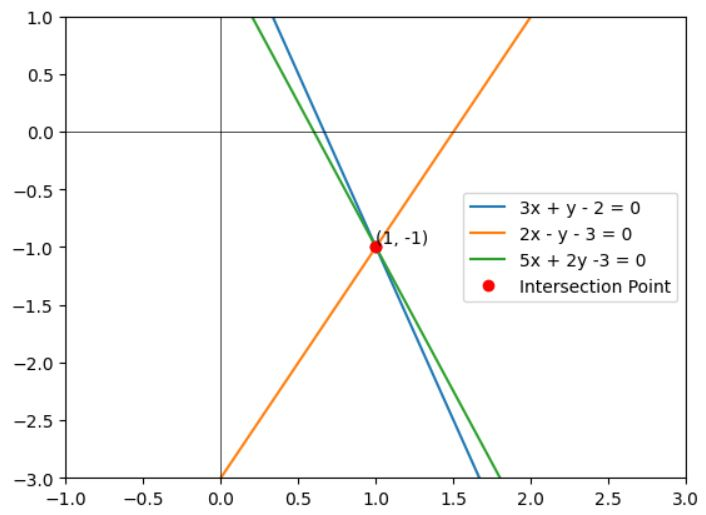
\includegraphics[width=\columnwidth]{figs/graph.jpg}
	\caption{Straight-lines}
	\label{fig:st.lines}
\end{figure}
\end{document}
